\documentclass[12pt,a4paper]{article}

\input{../../preamble_files/packages}
\input{../../preamble_files/scriptr}
\input{../../preamble_files/siunits}
\input{../../preamble_files/vectors}
\input{../../preamble_files/figures}
\input{../../preamble_files/references}

\pagestyle{fancy}
\lhead{Richard Whitehill}
\chead{PHYS 631 -- HW C}
\rhead{01/27/22}
\cfoot{\thepage \hspace{1pt} of \pageref{LastPage}}


\newcommand{\prob}[2]{\textbf{#1)} #2}

\setlength{\parskip}{\baselineskip}
\setlength{\parindent}{0pt}

\begin{document}

\prob{1.37}{Find formulas for $r,\theta,\phi$ in terms of $x,y,z$.}

The equations changing $(r,\theta,\phi)$ to $(x,y,z)$ are
\begin{align*}
\begin{cases}
x = r\cos{\phi}\sin{\theta} \\
y = r\sin{\phi}\sin{\theta} \\
z = r\cos{\theta}
\end{cases}
\end{align*}
It is obvious that
\begin{align*}
x^2 + y^2 + z^2 = r^2\cos^2{\phi}\sin^2{\phi} + r^2\sin^2{\phi}\sin^2{\theta} + r^2\cos^2{\theta} = r^2,
\end{align*}
or
\begin{empheq}[box=\fbox]{align*}
r = \sqrt{x^2 + y^2 + z^2}
\end{empheq}

Then, it is seen that
\begin{empheq}[box=\fbox]{align*}
\theta = \arccos{\qty(\frac{z}{\sqrt{x^2 + y^2 + z^2}})}
\end{empheq}
and finally that
\begin{align*}
\frac{r\sin{\phi}\sin{\theta}}{r\cos{\phi}\sin{\theta}} = \tan{\phi} = \frac{y}{x}
\end{align*}
\begin{empheq}[box=\fbox]{align*}
\phi = \arctan{\qty(\frac{y}{x})}
\end{empheq}

\prob{1.41}{Compute the gradient and Laplacian of the function $T = r\qty(\cos{\theta} + \sin{\theta}\cos{\phi})$. Check the Laplacian by converting $T$ to Cartesian coordinates. Test the gradient theorem for this function, using the path shown in Fig. 1.41, from $(0,0,0)$ to $(0,0,2)$.}

Observer that
\begin{align*}
\laplacian T(r,\theta,\phi) &= \frac{1}{r^2}\frac{\partial}{\partial r}\qty(r^2\frac{\partial T}{\partial r}) + \frac{1}{r^2\sin{\theta}}\frac{\partial}{\partial \theta}\qty(\sin{\theta}\frac{\partial T}{\partial \theta}) + \frac{1}{r^2\sin^2{\theta}}\frac{\partial^2 T}{\partial \phi^2} \\
&= \frac{1}{r^2}\frac{\partial}{\partial r}\qty(r^2)\qty(\cos{\theta} + \sin{\theta}\cos{\phi}) + \frac{1}{r\sin{\theta}}\frac{\partial}{\partial \theta}\qty(-\sin^2{\theta}\cos{\theta}\sin{\theta}\cos{\phi}) + \frac{1}{r^2\sin^2{\theta}}\qty(-\cos{\phi}) \\
&= \frac{2\qty(\cos{\theta} + \sin{\theta}\cos{\phi})}{r} + \frac{-\sin^2{\theta}\cos{\phi} - 2\sin{\theta}\cos{\theta} + \cos^2{\theta}\cos{\phi}}{r\sin{\theta}} - \frac{\cos{\phi}}{r\sin{\theta}}
\end{align*}
\begin{empheq}[box=\fbox]{align*}
\laplacian T = 0
\end{empheq}

In Cartesian coordinates 
\begin{align*}
T = \sqrt{x^2 + y^2 + z^2}\qty(\frac{z}{\sqrt{x^2 + y^2 + z^2}} + \frac{\sqrt{x^2 + y^2}}{\sqrt{x^2 + y^2 + z^2}}\frac{x}{\sqrt{x^2 + y^2 + z^2}}) = z + x
\end{align*}
Clearly, then
\begin{empheq}[box=\fbox]{align*}
\laplacian T = 0
\end{empheq}

The gradient theorem states $\int_{C} \grad T \cdot \dd \vec{l} = T(B) - T(A)$, and the path $C$ is shown below.
\bef
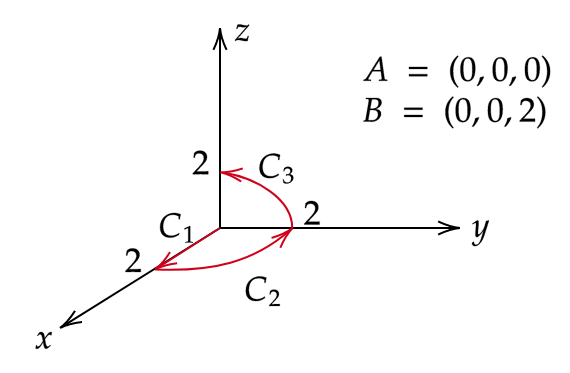
\includegraphics[scale=0.5]{./fig1.png}
\eef
Note that $C = C_1 + C_2 + C_3$, so $\int_{C} = \int_{C_1} + \int_{C_2} + \int_{C_3}$, and $\grad T = \gradsph[T]$.
Hence, since $\dd{\va*{l}} = \dlsph$, then
\begin{align*}
\int_C \grad{T} \vdot \dd{\va*{l}} = \int_C \qty(\cos{\theta} + \sin{\theta}\cos{\phi})\dd{r} + \int_C r\qty(-\sin{\theta} + \cos{\theta}\cos{\phi})\dd{\theta} + \int_C r\sin{\theta}\qty(-\sin{\phi})\dd{\phi}
\end{align*}
The integrals over each path are as follows:
\begin{align*}
\int_{C_1} \grad{T} \vdot \dd{\va*{l}} &= \qty(\cos(\frac{\pi}{2}) + \sin(\frac{\pi}{2})\cos(0))(2) = 2 \\
\int_{C_2} \grad{T} \vdot \dd{\va*{l}} &= -2\sin(\frac{\pi}{2})\int_{0}^{\pi/2} \sin{\phi}\dd{\phi} = -2 \\
\int_{C_3} \grad{T} \vdot \dd{\va*{l}} &= 2\int_{\pi/2}^{0} \qty(-\sin{\phi})\dd{\phi} = 2
\end{align*}
Summing up the contribution over each part, we see that
\begin{empheq}[box=\fbox]{align*}
\int_{C} \grad{T} \vdot \dd{\va*{l}} &= 2,
\end{empheq}
which is the same as given by the right hand side of the gradient theorem
\begin{empheq}[box=\fbox]{align*}
T(0,0,2) - T(0,0,0) = 2 - 0 = 0.
\end{empheq}

\prob{1.44}{Evaluate the following integrals:}

(a) $\int_{2}^{6} \qty(3x^2 - 2x - 1)\delta\qty(x-3)\dd{x} = 3(3)^2 - 2(3) - 1 = \boxed{20}$

(b) $\int_{0}^{5} \cos{x}\delta\qty(x-\pi)\dd{x} = \cos{\pi} = \boxed{-1}$

(c) $\int_{0}^{3} x^3\delta\qty(x+1)\dd{x} = \boxed{0}$

(d) $\int_{-\infty}^{\infty} \ln(x+3)\delta\qty(x+2)\dd{x} = \ln(-2 + 3) = \boxed{0}$

\end{document}
